\documentclass[11pt,a4paper]{article}

% ---------------------------------------------------------------------------
%  SupplyForge -- technical note: what the package does and its core assumptions
%  Author: Simon Brigode <simon.brigode@ehess.fr>
%  Builds on supplyforge by Yassine Abdelouadoud.
% ---------------------------------------------------------------------------

\usepackage[utf8]{inputenc}
\usepackage[T1]{fontenc}
\usepackage{lmodern}
\usepackage[a4paper,margin=2.4cm]{geometry}
\usepackage{amsmath}
\usepackage{booktabs}
\usepackage{array}
\usepackage{xcolor}
\usepackage{graphicx}
\usepackage{caption}
\usepackage{enumitem}
\usepackage{fancyhdr}
\usepackage{listings}
\usepackage{tikz}
\usetikzlibrary{positioning,fit,backgrounds,arrows.meta}
\usepackage[hidelinks,colorlinks=true,linkcolor=blue!50!black,urlcolor=blue!50!black,citecolor=blue!50!black]{hyperref}

% --- running header ---
\pagestyle{fancy}
\fancyhf{}
\lhead{\small SupplyForge --- multi-area model \& assumptions}
\rhead{\small\thepage}
\renewcommand{\headrulewidth}{0.4pt}

% --- code listings (gray boxes) ---
\definecolor{codebg}{gray}{0.95}
\lstset{
  basicstyle=\ttfamily\small,
  backgroundcolor=\color{codebg},
  frame=single, framerule=0pt, rulecolor=\color{codebg},
  breaklines=true, columns=fullflexible, keepspaces=true,
  xleftmargin=6pt, xrightmargin=6pt, aboveskip=8pt, belowskip=8pt,
}
\newcommand{\code}[1]{\lstinline[basicstyle=\ttfamily]|#1|}

% --- TikZ box styles ---
\tikzset{
  srcbox/.style ={rectangle, rounded corners, draw=blue!55,   fill=blue!8,   align=center, inner sep=3pt, minimum height=8mm, text width=23mm, font=\footnotesize},
  fetchbox/.style={rectangle, rounded corners, draw=green!55!black, fill=green!10, align=center, inner sep=3pt, minimum height=8mm, text width=27mm, font=\footnotesize},
  procbox/.style ={rectangle, rounded corners, draw=orange!75!black, fill=orange!12, align=center, inner sep=3pt, minimum height=8mm, text width=27mm, font=\footnotesize},
  modelbox/.style={rectangle, rounded corners, draw=red!60,    fill=red!8,    align=center, inner sep=3pt, minimum height=8mm, text width=29mm, font=\footnotesize},
  exbox/.style   ={rectangle, rounded corners, draw=violet!60, fill=violet!10, align=center, inner sep=3pt, minimum height=8mm, text width=27mm, font=\footnotesize},
  flow/.style    ={-{Latex[length=2mm]}, draw=black!55, thick},
}

\title{\textbf{SupplyForge --- a multi-area European power \& hydrogen model}\\[2pt]
\large What the package does, its data pipeline, and its core assumptions}
\author{Simon Brigode \quad\textendash\quad \texttt{simon.brigode@ehess.fr}}
\date{8 June 2026}

\begin{document}
\maketitle
\thispagestyle{fancy}

\begin{abstract}
\noindent SupplyForge is a Python package that (i) downloads and harmonises European weather and
power-system data and (ii) assembles them into runnable \texttt{pommes\_craft} (linopy + HiGHS)
optimisation models. This note describes the whole package --- the \texttt{fetch}/\texttt{process}
data pipeline, the multi-area model builder, and the physical and economic assumptions --- and walks
through three worked examples (a single-node-per-country European greenfield model, a France--Belgium
regional electricity\,+\,hydrogen case, and a small NUTS-2 demonstrator). It is a reference for the
modelling layer, not a study: copper-plate nodes, illustrative demand levels and a representative-hour
sample are used where noted.
\end{abstract}

\tableofcontents
\bigskip

% ===========================================================================
\section{Purpose of this document}
This note documents \textbf{SupplyForge}: what it does, how its layers fit together, and the
assumptions baked into the models it produces. It is aimed at a reader who wants to understand or
re-use the package without reading every module. The four goals are to:
\begin{enumerate}[nosep]
  \item describe the four-layer architecture (\texttt{fetch} $\to$ \texttt{process} $\to$ model-build
        $\to$ examples) and the role of each part;
  \item document the data sources and how they are harmonised;
  \item formalise the physical and economic assumptions (costs, lifetimes, annualisation, weather);
  \item walk through the worked example models and their results.
\end{enumerate}

% ===========================================================================
\section{What SupplyForge does}
SupplyForge couples a \textbf{Snakemake data workflow} with a \textbf{model generator}. The workflow
acquires raw data from external providers (PECD~4.2 via the Copernicus CDS, ENTSO-E Transparency, the
ERAA~2024 study, OpenStreetMap, Ember) and processes it into a small set of canonical, per-country
hourly Parquet files (capacity factors, hydro inflow, availability, installed capacity, net-transfer
capacities). The model layer then turns those files --- plus user scenario assumptions --- into a
\texttt{pommes\_craft} \texttt{EnergyModel} that can be solved with HiGHS to obtain a least-cost
dispatch and/or capacity-expansion solution.

The design separates two kinds of inputs cleanly: \emph{weather and grid data} (reproducible, fetched)
versus \emph{scenario assumptions} (fleet, demand, costs --- supplied by the caller). The same builder
serves both \emph{country} nodes and finer \emph{NUTS-2} nodes; it is node-agnostic.

% ===========================================================================
\section{Architecture}
Four layers, each depending only on the one before it (Figure~\ref{fig:arch}).
\begin{itemize}[nosep]
  \item \textbf{\texttt{fetch/}} --- acquisition of raw data from external sources; minimal cleaning,
        on-disk caching, returns DataFrames.
  \item \textbf{\texttt{process/}} --- harmonisation into canonical hourly series (capacity factors,
        inflow, availability), with consistent schemas across data sources.
  \item \textbf{model build} --- \texttt{grid\_model.py} (multi-area) and
        \texttt{create\_pommes\_craft\_model.py} (country-level) assemble a \texttt{pommes\_craft}
        model from processed data + assumptions.
  \item \textbf{examples} --- \texttt{scripts/} and \texttt{notebooks/} assemble inputs, solve, and
        visualise.
\end{itemize}

\begin{figure}[ht]
\centering
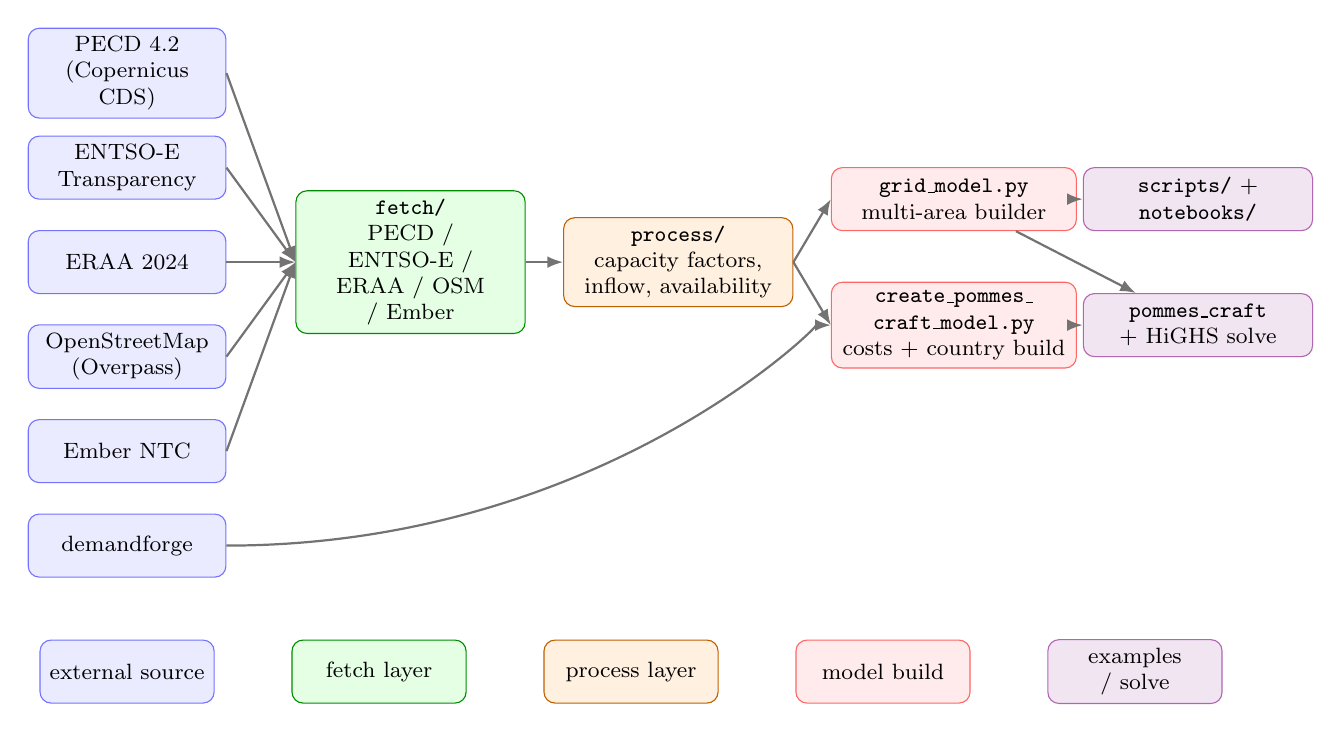
\begin{tikzpicture}
% --- column 1: external sources ---
\node[srcbox] (pecd)  at (0,4.2) {PECD 4.2\\(Copernicus CDS)};
\node[srcbox] (entsoe)at (0,3.0) {ENTSO-E\\Transparency};
\node[srcbox] (eraa)  at (0,1.8) {ERAA 2024};
\node[srcbox] (osm)   at (0,0.6) {OpenStreetMap\\(Overpass)};
\node[srcbox] (ember) at (0,-0.6){Ember NTC};
\node[srcbox] (df)    at (0,-1.8){demandforge};
% --- column 2: fetch ---
\node[fetchbox] (fetch) at (3.6,1.8) {\texttt{fetch/}\\PECD / ENTSO-E /\\ERAA / OSM / Ember};
% --- column 3: process ---
\node[procbox] (proc) at (7.0,1.8) {\texttt{process/}\\capacity factors,\\inflow, availability};
% --- column 4: model ---
\node[modelbox] (grid) at (10.5,2.6) {\texttt{grid\_model.py}\\multi-area builder};
\node[modelbox] (cpm)  at (10.5,1.0) {\texttt{create\_pommes\_}\\\texttt{craft\_model.py}\\costs + country build};
% --- column 5: examples / solve ---
\node[exbox] (ex) at (13.6,2.6) {\texttt{scripts/} +\\\texttt{notebooks/}};
\node[exbox] (solve) at (13.6,1.0) {\texttt{pommes\_craft}\\+ HiGHS solve};
% --- arrows ---
\foreach \s in {pecd,entsoe,eraa,osm,ember} {\draw[flow] (\s.east) -- (fetch.west);}
\draw[flow] (fetch) -- (proc);
\draw[flow] (proc.east) -- (grid.west);
\draw[flow] (proc.east) -- (cpm.west);
\draw[flow] (df.east) .. controls (6,-1.8) and (8.8,1.0) .. (cpm.west);
\draw[flow] (grid) -- (ex);
\draw[flow] (grid) -- (solve);
\draw[flow] (cpm) -- (solve);
% --- legend ---
\begin{scope}[shift={(0,-3.4)}]
  \node[srcbox,   text width=20mm] (l1) at (0,0)   {external source};
  \node[fetchbox, text width=20mm] (l2) at (3.2,0) {fetch layer};
  \node[procbox,  text width=20mm] (l3) at (6.4,0) {process layer};
  \node[modelbox, text width=20mm] (l4) at (9.6,0) {model build};
  \node[exbox,    text width=20mm] (l5) at (12.8,0){examples / solve};
\end{scope}
\end{tikzpicture}
\caption{SupplyForge architecture: external sources are fetched, harmonised, then assembled into a
\texttt{pommes\_craft} model and solved. \texttt{demandforge} supplies hydrogen and electricity demand
directly to the model layer.}
\label{fig:arch}
\end{figure}

% ===========================================================================
\section{Data acquisition (\texttt{fetch/})}
The \texttt{fetch} layer (33 modules) acquires raw data and caches it on disk. Table~\ref{tab:sources}
lists the providers.

\begin{table}[ht]
\centering
\caption{External data sources.}
\label{tab:sources}
\small
\begin{tabular}{@{}lll@{}}
\toprule
\textbf{Source} & \textbf{What it provides} & \textbf{Used for} \\
\midrule
PECD 4.2 (Copernicus CDS) & solar/wind capacity factors, hydro inflow & weather inputs (historical + projections) \\
ENTSO-E Transparency      & generation, capacity, prices, outages    & historical CF, availability, border prices \\
ERAA 2024                 & prospective CF + storage volumes         & future-year weather, reservoir energy \\
OpenStreetMap (Overpass)  & power plants, grid, industrial land use   & regional fleet \& grid/demand context \\
Ember                     & cross-border net-transfer capacities      & interconnection limits \\
demandforge               & electricity load + industrial H$_2$ demand & demand profiles \& hydrogen demand \\
Eurostat GISCO            & NUTS / country geometry                    & maps + region adjacency \\
\bottomrule
\end{tabular}
\end{table}

\paragraph{PECD 4.2.} Fetched per a configuration dict selecting the climate model (\texttt{origin},
e.g.\ EC-Earth3), emission scenario (\texttt{ssp1\_2\_6} \dots \texttt{ssp5\_8\_5}), spatial resolution
(\texttt{szon} bidding zones, \texttt{p2on}/\texttt{p2of} wind, or \texttt{nuts\_2} for solar) and
climate years. \texttt{ssp2\_4\_5} is the median scenario.

\paragraph{OpenStreetMap.} A cache-first, multi-mirror Overpass client (\texttt{fetch/osm/}) turns OSM
tags into per-NUTS-region aggregates: power plants ($\to$ capacity by technology), substations/converters
($\to$ grid nodes), lines/cables ($\to$ circuit-km by voltage), and industrial land use ($\to$ a
demand-side proxy). Data \textcopyright{} OpenStreetMap contributors (ODbL).

% ===========================================================================
\section{Data processing (\texttt{process/})}
The \texttt{process} layer (15 modules) harmonises raw data into canonical hourly series with a common
schema, so that PECD, ERAA and ENTSO-E inputs are interchangeable downstream. It computes hourly
capacity factors, reconstructs hydro inflow, derives availability from outage events, and aggregates
zonal PECD data to the country level.

\paragraph{Zonal aggregation.} PECD reports at bidding-zone resolution. A country's national capacity
factor is the \emph{installed-capacity-weighted} average over its zones $z$:
\begin{equation}
\mathrm{CF}_{\text{nat}}(t) \;=\; \frac{\sum_z \mathrm{CF}_z(t)\,C_z}{\sum_z C_z},
\label{eq:cf}
\end{equation}
with weights $C_z$ from a configured per-zone capacity table (equal weights as a logged fallback). All
series are leap-trimmed to exactly 8760~hours and clipped to $[0,1]$.

\paragraph{Source resolution.} \texttt{sources.py} resolves which engine supplies each input
(\texttt{res\_source}~$\in$~\{\texttt{entsoe}, \texttt{era5}, \texttt{pecd}\}; hydro and run-of-river
resolved independently), so weather provenance is an orthogonal configuration choice.

% ===========================================================================
\section{Physical and economic assumptions}
\subsection{Cost basis}
Costs live in \texttt{create\_pommes\_craft\_model.py} (Table~\ref{tab:costs}): overnight CAPEX,
fixed O\&M, short-run variable cost, and technical life per technology. These are the values the
greenfield expansion uses.

\begin{table}[ht]
\centering
\caption{Cost and lifetime basis (selected technologies).}
\label{tab:costs}
\small
\begin{tabular}{@{}lrrrr@{}}
\toprule
\textbf{Technology} & \textbf{CAPEX} & \textbf{Fixed O\&M} & \textbf{Variable} & \textbf{Life} \\
                    & (kEUR/MW) & (kEUR/MW/yr) & (EUR/MWh) & (yr) \\
\midrule
Solar PV          & 700  & 12  & 0   & 25 \\
Wind onshore      & 1300 & 35  & 0   & 25 \\
Wind offshore     & 3200 & 85  & 0   & 25 \\
Nuclear           & 7500 & 120 & 10  & 60 \\
Gas (CCGT)        & 900  & 20  & 200 & 30 \\
Biomass           & 3500 & 60  & 50  & 25 \\
Hard coal         & 1800 & 45  & 250 & 40 \\
Oil               & 500  & 25  & 300 & 30 \\
Reservoir hydro   & 4000 & 30  & --- & 80 \\
Electrolyser      & 155  & 12  & --- & 10 \\
\bottomrule
\end{tabular}
\end{table}

\subsection{Annuities and the decommission horizon}
Investment costs are annualised with the capital-recovery factor
\begin{equation}
\mathrm{CRF}(n,r) \;=\; \frac{r\,(1+r)^n}{(1+r)^n - 1}, \qquad r = 0.04,
\label{eq:crf}
\end{equation}
for a technology of life $n$ years. The multi-area model keeps a \emph{single} decommission year
($\text{model year}+25$) to bound LP memory, which forces every investable technology to declare
\texttt{life\_span}=25. To still annualise each technology over its \emph{true} life, the overnight
CAPEX is rescaled
\begin{equation}
\widetilde{\mathrm{CAPEX}} \;=\; \mathrm{CAPEX}\,\cdot\,\frac{\mathrm{CRF}(\text{life})}{\mathrm{CRF}(25)},
\label{eq:rescale}
\end{equation}
so the 25-year annuity computed by \texttt{pommes\_craft} equals the real-life annuity (e.g.\ nuclear
is annualised over 60~years, not 25). The economy-wide discount rate is 0 (an energy-planning
convention); the per-technology finance rate $r=0.04$ governs the annuity.

\subsection{Representative-hour annualisation}
The power balance holds at face value each modelled hour (\texttt{time\_step\_duration}=1.0), while
costs and energy are annualised over \texttt{operation\_year\_duration}=8760. A sample of $H<8760$ hours
therefore stands for the whole year, each modelled hour weighted $8760/H$:
\begin{equation}
\text{annual energy} \;=\; \sum_{h=1}^{H} P_h \,\cdot\, \frac{8760}{H}.
\label{eq:annual}
\end{equation}
Because a non-contiguous representative sample breaks hour-to-hour coupling, inter-hour storage is
disabled in that mode; firm dispatchable plant covers the residual.

% ===========================================================================
\section{The multi-area model (\texttt{grid\_model.py})}
\texttt{build\_grid\_model} assembles one \texttt{pommes\_craft} \texttt{Area} per node, connected by
bidirectional transport links. Each node carries an \texttt{assumptions} dict; the public API is small
(Table~\ref{tab:api}).

\begin{table}[ht]
\centering
\caption{Public API of \texttt{grid\_model.py}.}
\label{tab:api}
\small
\begin{tabular}{@{}ll@{}}
\toprule
\textbf{Function} & \textbf{Purpose} \\
\midrule
\texttt{build\_grid\_model(...)}    & build an \emph{unsolved} multi-area \texttt{EnergyModel} from explicit inputs \\
\texttt{build\_european\_grid(...)} & wrapper: PECD inputs + Ember links, then \texttt{build\_grid\_model} \\
\texttt{pecd\_country\_inputs(...)} & per-country capacity factors + hydro inflow from staged PECD CSVs \\
\texttt{ember\_ntc\_links(...)}     & de-duplicated cross-border NTCs as \texttt{(a, b, mw)} tuples \\
\texttt{grid\_flows(model)}         & after solve: hourly directional cross-border flows \\
\bottomrule
\end{tabular}
\end{table}

\paragraph{Per-node assumptions.} A node is described by a dict; the salient keys are:
\begin{lstlisting}
{
  "demand_TWh": 580,            # flat annual demand  (or "demand_profile": hourly MW array)
  "solar_GW": 60, "wind_onshore_GW": 40,            # fixed intermittent (availability = PECD CF)
  "firm": {"Nuclear": {"GW": 60, "cost": 10},       # fixed dispatchable, dispatched by merit order
           "Gas":     {"GW": 30, "cost": 200}},
  "greenfield": {"Solar": 600, "Wind_Onshore": 400, # OR: investable generation, optimiser-sized
                 "Nuclear": 63, "Gas": 300},
  "h2": {"efficiency": 0.70, "demand_MW": 4500,      # optional hydrogen layer (electrolyser + demand)
         "electrolyser_max_GW": 80, "storage": False},
}
\end{lstlisting}

\paragraph{Conventions.}
\begin{itemize}[nosep]
  \item \emph{Intermittent RE}: output $=$ capacity $\times$ availability (the hourly PECD CF), zero
        variable cost.
  \item \emph{Firm merit order}: each \texttt{firm} technology is priced at its short-run marginal cost,
        so HiGHS dispatches cheapest-first.
  \item \emph{NTC links}: a \texttt{pommes\_craft} \texttt{Link} is one-directional, so each border is
        \emph{two} one-way links (\texttt{a$\to$b}, \texttt{b$\to$a}), each capped at the NTC, with a
        small hurdle cost.
\end{itemize}

\paragraph{Greenfield expansion.} Setting \texttt{greenfield} makes generation investable, sized by the
optimiser using the cost basis of Table~\ref{tab:costs} and the annuity rescale of
Eq.~\eqref{eq:rescale}.

\paragraph{Hydrogen layer.} An \texttt{h2} config adds an \emph{investable electrolyser} (siting and
size chosen by the optimiser), optional H$_2$ demand and storage, and feasibility valves. The
electrolyser uses the sign convention
\begin{equation}
\text{factor} = \{\text{electricity}: -1,\ \text{hydrogen}: \eta\}, \qquad \eta = 0.70\ \text{MWh H}_2/\text{MWh}_e,
\end{equation}
(consumed negative, produced positive). Passing \texttt{h2\_links} adds an H$_2$ pipeline
\emph{backbone} so hydrogen can flow between nodes, letting electrolysis migrate to the
cheapest-power nodes.

% ===========================================================================
\section{The country-level builder (\texttt{create\_pommes\_craft\_model.py})}
The original single-country builder assembles a national model from staged inputs: fixed dispatchable
and intermittent fleets, reservoir and pumped hydro (each a storage\,+\,inflow\,+\,turbine assembly),
price-taking border imports (\texttt{add\_imports}: a \texttt{NetImport} priced by day-ahead prices,
capped at the NTC), and an optional hydrogen system (\texttt{add\_hydrogen}). It also defines the cost
dictionaries that the multi-area greenfield path imports.

% ===========================================================================
\section{Worked examples}
\subsection{Single node per country (greenfield 2050)}
\texttt{scripts/eu\_countries.py} builds one copper-plate node per country (16 core EU + CH/NO),
greenfield generation, a \emph{hypothetical} 2050 electricity demand dict, industrial hydrogen demand
(demandforge) served by electrolysis over a 30~GW H$_2$ backbone, PECD \texttt{ssp2\_4\_5} weather, and
Ember links. Nuclear is bounded per country as a policy proxy (Table~\ref{tab:caps}); without the cap a
cost-minimiser builds only nuclear (its all-in cost is the lowest firm option). Biomass is capped low
as a feedstock proxy.

\begin{table}[ht]
\centering
\caption{EU example: greenfield build limits (GW). Nuclear is per-country (policy); the rest are shared.}
\label{tab:caps}
\small
\begin{tabular}{@{}lr@{\hskip 18pt}lr@{}}
\toprule
\textbf{Shared limit} & \textbf{GW} & \textbf{Nuclear cap} & \textbf{GW} \\
\midrule
Solar         & 600 & France         & 63 \\
Wind onshore  & 400 & Sweden         & 10 \\
Gas           & 300 & Poland         & 9 \\
Biomass       & 5   & Czechia        & 6 \\
              &     & Finland        & 6 \\
              &     & Netherlands    & 5 \\
              &     & Switzerland    & 3 \\
              &     & (others)       & 0 \\
\bottomrule
\end{tabular}
\end{table}

A representative-hour solve (16 countries, 96 hours) gives a renewables-led mix --- wind dominant in
the north, solar in the south, French nuclear, gas as backup --- and, with the H$_2$ backbone,
electrolysis concentrates in the cheapest-power countries (Iberia, the Nordics) while Germany imports
most of its hydrogen (Figures~\ref{fig:cap}--\ref{fig:h2}).

\begin{figure}[ht]
\centering
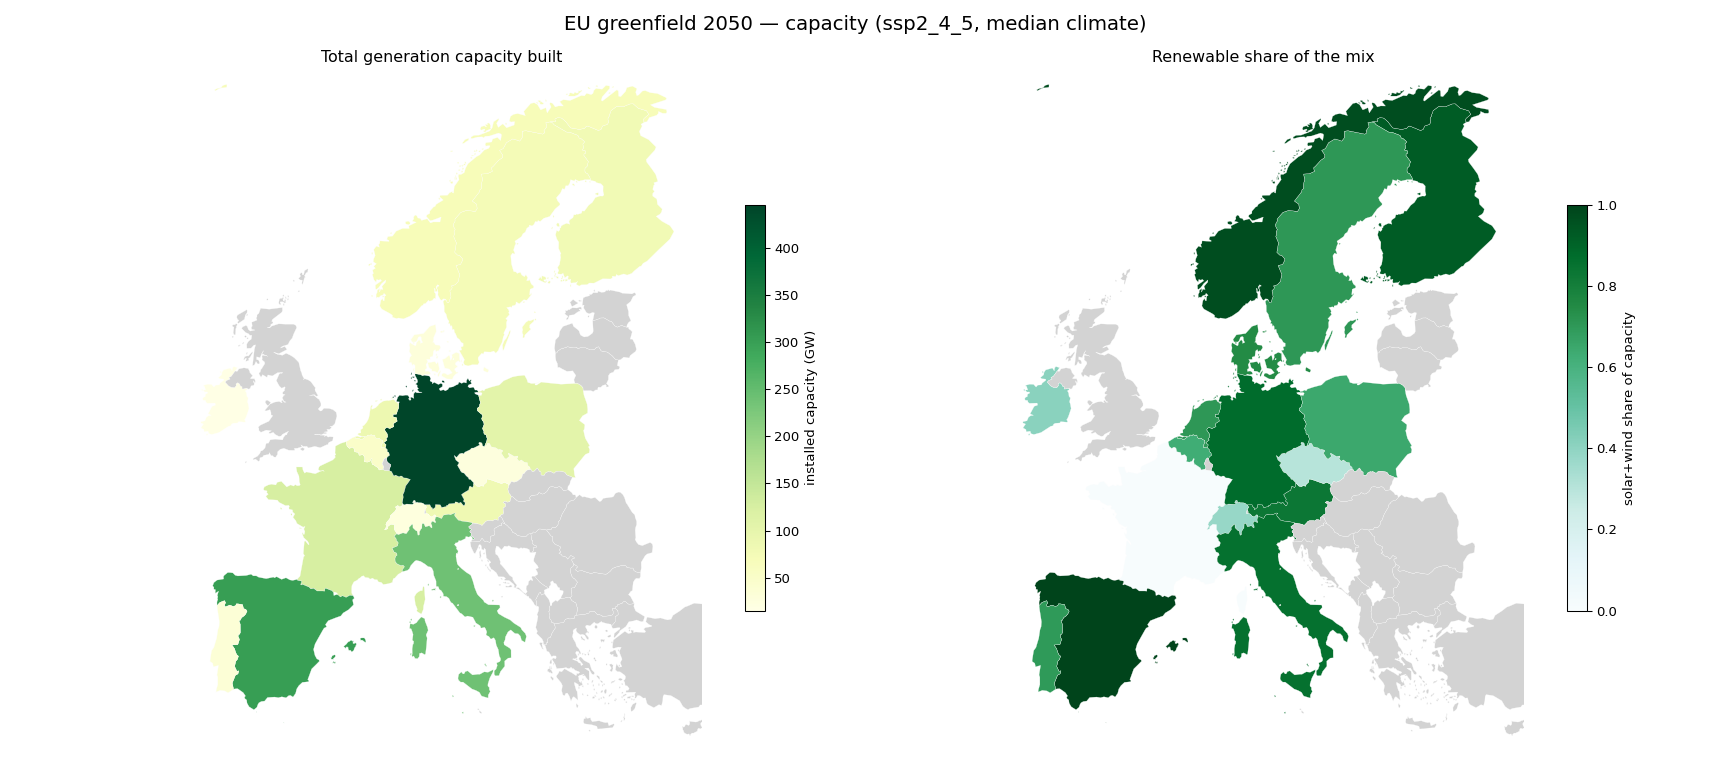
\includegraphics[width=\textwidth]{figs/capacity.png}
\caption{Total installed capacity (left) and renewable share of capacity (right) per country.}
\label{fig:cap}
\end{figure}

\begin{figure}[ht]
\centering
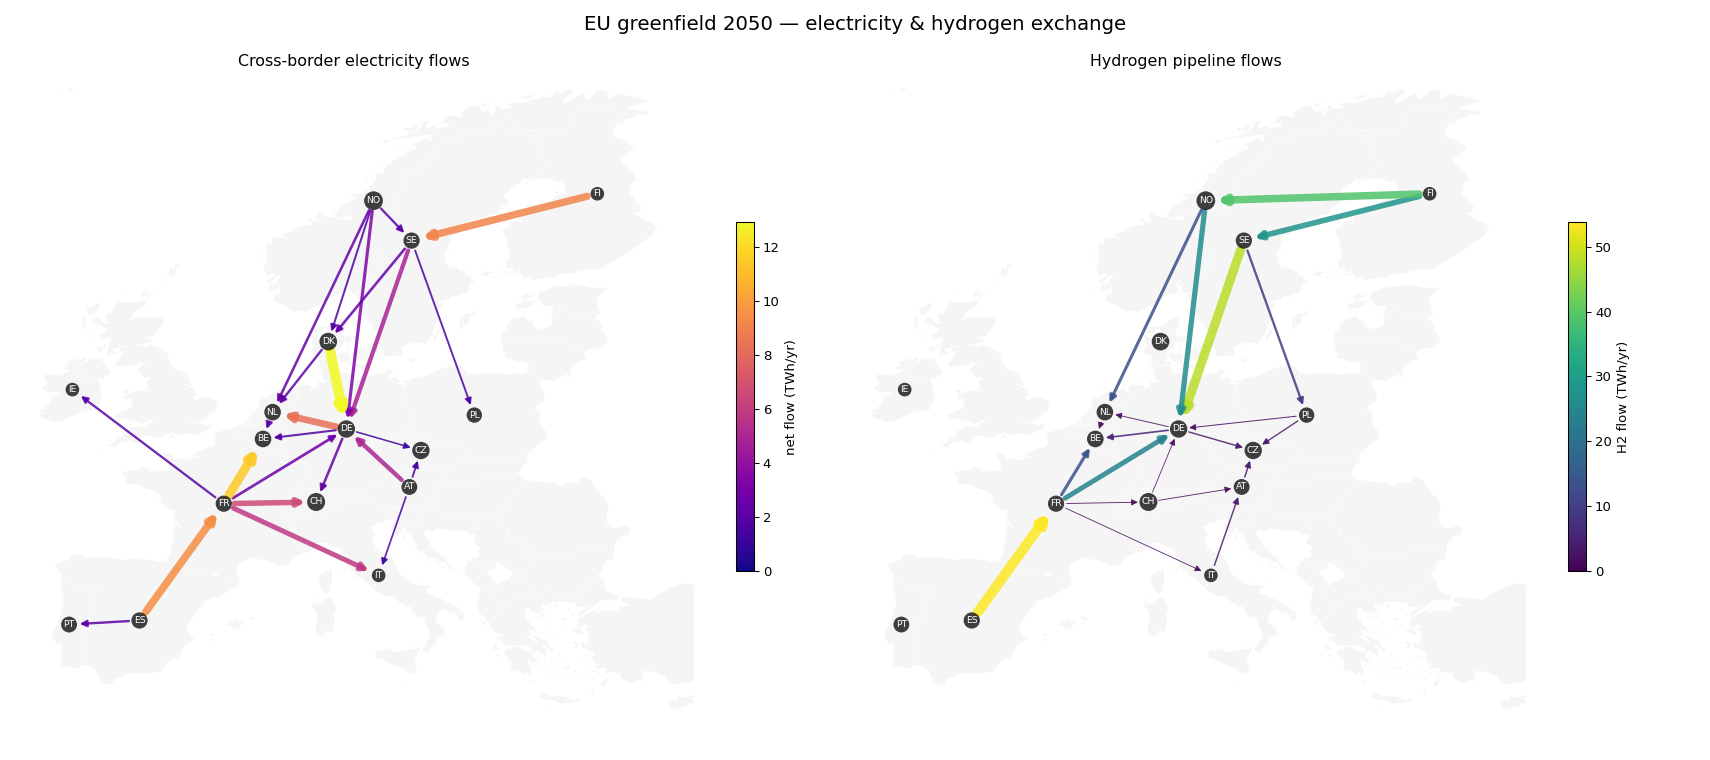
\includegraphics[width=\textwidth]{figs/flows.png}
\caption{Cross-border net flows: electricity (left) and the hydrogen backbone (right).}
\label{fig:flows}
\end{figure}

\begin{figure}[ht]
\centering
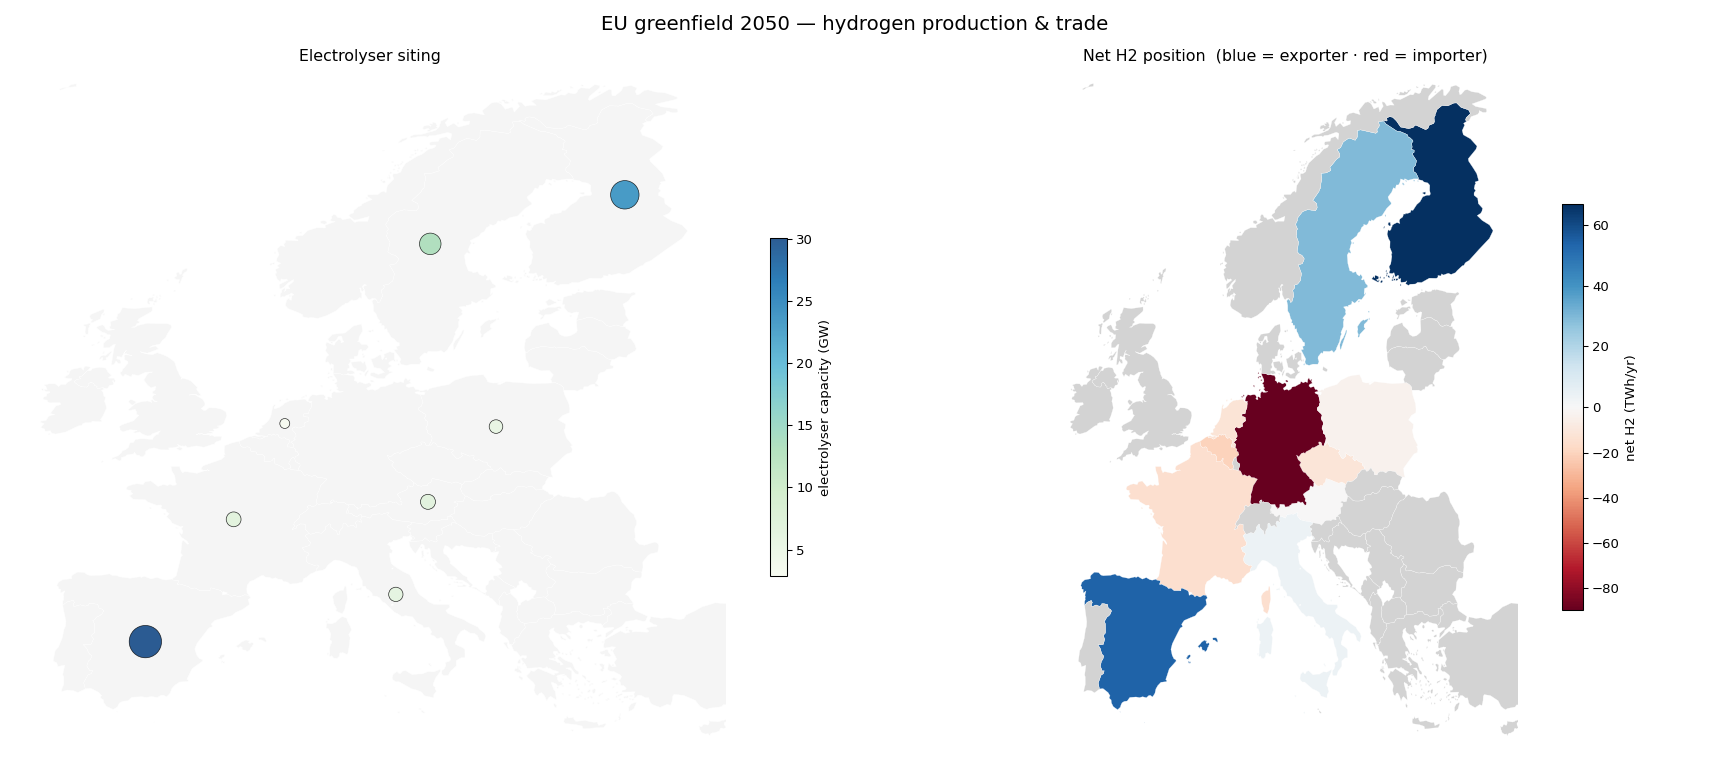
\includegraphics[width=\textwidth]{figs/hydrogen.png}
\caption{Hydrogen: electrolyser siting (left) and net H$_2$ position per country (right; blue~=~exporter,
red~=~importer).}
\label{fig:h2}
\end{figure}

\subsection{France--Belgium regional electricity + hydrogen}
\texttt{scripts/fr\_be\_h2.py} co-optimises FR+BE NUTS-2 nodes: electricity demand from demandforge
(disaggregated to NUTS-2 by area share), generation from PECD NUTS-2 solar + national wind + the OSM
fleet priced in merit order, and an industrial hydrogen network with demand at five weighted hubs
(Dunkerque, Fos, Toulouse; Antwerp, Ghent), investable electrolysers at every node, H$_2$ pipelines,
and H$_2$ storage. It demonstrates electrolysis siting and H$_2$ routing toward the demand hubs.

\subsection{Small NUTS-2 demonstrator}
\texttt{scripts/regional\_fr\_de\_be.py} is a minimal FR/DE/BE cross-border NUTS-2 example: real PECD
NUTS-2 solar and GISCO geometry/adjacency; wind, demand and fleet split per region by area; Ember
country NTC split over border-region pairs (all assumptions logged).

% ===========================================================================
\section{Weather configuration and scenarios}
The examples use PECD \texttt{ssp2\_4\_5} (median climate), EC-Earth3, climate year 2050, with solar at
\texttt{szon} (or \texttt{nuts\_2} for the regional case) and onshore wind at \texttt{p2on}. Other
climate models, emission scenarios (\texttt{ssp1\_2\_6}\dots\texttt{ssp5\_8\_5}) and climate years are
available by changing the configuration dict; national capacity factors are then aggregated via
Eq.~\eqref{eq:cf}.

% ===========================================================================
\section{Verification and guardrails}
\begin{itemize}[nosep]
  \item \textbf{Tests} --- 124 tests across the fetch, process, model and hydrogen layers
        (\texttt{supplyforge/tests/}).
  \item \textbf{Compilation} --- every module imports and passes \texttt{py\_compile}.
  \item \textbf{Feasibility} --- load-shedding/spillage valves make every node feasible; their use is a
        diagnostic.
  \item \textbf{Caveats} --- copper-plate nodes ignore intra-node grid limits; the representative-hour
        sample is not seasonally contiguous (no storage in that mode); the LP cost grows roughly as
        $\mathcal{O}(\text{nodes}^2 \times \text{links}^2)$, so dense all-pairs topologies are the
        binding memory constraint (a sparse Ember/backbone topology keeps it tractable).
\end{itemize}

% ===========================================================================
\section{File inventory}
\begin{table}[ht]
\centering
\caption{Python file inventory by layer.}
\label{tab:inv}
\small
\begin{tabular}{@{}lrrl@{}}
\toprule
\textbf{Layer} & \textbf{Files} & \textbf{Lines} & \textbf{Role} \\
\midrule
\texttt{supplyforge/} (root) & 6  & 2\,521 & model builders, cost basis, utils, results \\
\texttt{fetch/}              & 33 & 4\,970 & data acquisition (PECD, ENTSO-E, ERAA, OSM, Ember) \\
\texttt{process/}            & 15 & 2\,806 & harmonisation (capacity factors, inflow, availability) \\
\texttt{tests/}              & 20 & 1\,417 & 124 tests across all layers \\
\texttt{scripts/}            & 4  & 985    & worked example models \\
\midrule
\textbf{Total}               & \textbf{78} & \textbf{12\,699} & \\
\bottomrule
\end{tabular}
\end{table}

Key modules: \texttt{grid\_model.py} (423 lines), \texttt{create\_pommes\_craft\_model.py}
(1\,440), \texttt{eu\_countries.py} (351), \texttt{fr\_be\_h2.py} (323). The internal dependency graph
is acyclic --- \texttt{process} depends only on numpy/pandas/polars, model builders depend on
\texttt{process} + \texttt{pommes\_craft}, examples depend on the builders.

% ===========================================================================
\section{Credits and license}
The multi-area model layer (\texttt{grid\_model.py}), the worked examples (\texttt{scripts/}), the
OpenStreetMap fetchers (\texttt{fetch/osm/}) and the mapping toolkit
(\texttt{fetch/tools/visualisation/maps.py}) were written by \textbf{Simon Brigode}
(\texttt{simon.brigode@ehess.fr}). They build on \textbf{SupplyForge} and its data pipeline, cost
basis (\texttt{create\_pommes\_craft\_model.py}) and PECD/ENTSO-E integration by \textbf{Yassine
Abdelouadoud} (\texttt{yassine.abdelouadoud@minesparis.psl.eu}). The package is released under the MIT
license. OpenStreetMap data is \textcopyright{} OpenStreetMap contributors (ODbL); PECD data is from the
Copernicus Climate Data Store.

\end{document}
